\subsection{Hagen-Poiseuille Flow}
\section{Summary}

\clearpage
\clearpage

\subsection{Hagen-Poiseuille Flow}

\subsubsection{Theoretical description}

In the previous test case the channel walls were aligned parallel to the simulation grid, hence no further interpolation procedures
were necessary. In order to test the accuray of the interpolation methods, we now introduce a test case with a curved geometry.
Furthermore we have the possibility to investigate the error of non-interpolating methods on curved surfaces.\\
The most simplest extension of the planar poiseuille flow, is the laminar flow through a pipe,
also referred to as Hagen-Poiseuille flow. The setup of the fluid domain is schematically shown in Fig. ().
We consider a flow in z-Direction where the total size of the simulation domain is set to $L_x = L_y = L$.
The immersed boundary is restricted by a wall at the radius $r_0=0.4L$ where r is defined as the distance from the pipe center $\vec{m} = (L/2, L/2)^T$.
The length $L_z$ can be chosen arbitrary due to the flow invariance in z direction.\\
\begin{figure}[!bp]
  \centering
  \includegraphics[width=0.8\textwidth]{gfx/immersed_boundary/val_volpen/poiseuilleflow.png}\label{b}
  \caption{Theoretical setup of the poiseuille-flow channel.}
\end{figure}
For an analytical solution of this problem we referr to [CITEFLUID].
Once again we can assume a steady state flow which implies $\partial v_z/\partial t = 0$. With the introduction of cylindrical coordinates $(r, \phi, x)$
and the assumption that the flow is independent of $\phi$ the equation of motion reduces to
\begin{align}
        0 &= - \frac{\partial p}{\partial x}  +  \frac{\nu}{r}\frac{\partial}{\partial r}\left(r\frac{\partial u}{\partial r}\right)
\end{align}
The solution is obtained by seperation of variables and integrating twice.
\begin{align}
    u &= \frac{r^2}{4\nu}\frac{\partial p}{\partial x} + A \ln r + B
\end{align}
By using the boundarie conditions $u(r_0) = 0$ and choose the same non-dimensionalization as in section (), with the expection of setting the length scale to $r_0$,
the velocity profile for the channel is given by
\begin{align}
    u &= \frac{r^2 - r_0^2}{4}\frac{\partial p}{\partial x}Re
\end{align}
Since $v_{max} \stackrel{!}{=} 1$ by definition, the pressure condition for the domain needs to be set to
\begin{align}
    \frac{\partial p}{\partial x} = -\frac{4 r_o^2}{Re}
\end{align}

\subsubsection{Grid Convergence Study}

For an error evaluation a grid convergence study was performed, for a constant reynolds number of $Re=100$.
The number of grid points was varied in the intervall $N\in[32, 256]$ with a stepsize of $\Delta N = 16$, furthermore a
simulation with a resolution of $N=512$ was carried out.\\
Since the maximum velocity of the channel is given by $v_{max}=1$, due to the choice of non-dimensionalization,
the sound speed was set to $c^2 = 100$ to fullfill the incompressibilty condition $Ma = v/c < 0.1$. \footnote{In order to exclude
any influence of choice of the sound speed on the resulting error, further simulations were carried out with a diffent $c^2$ and will be discussed}
With this choice the cfl-condition for the system is given by $\Delta t < \min(\Delta x^2 \cdot Re, \Delta x / 10)$.
The resulting timestep for the highest resolution is $\Delta t = 1e-4$.
With the above defined setup all methods introduced in section were tested, for 2nd and 4th order finite difference stencils.\\
For the penalization method the non-dimensionalized damping was set to $J=1e-4$.
It would be possible to choose a larger time step for the lower resolution cases, which means that in general
one would apply a smaller damping rate $J$ in a case of applicaton. To remain consistent in the error convergence, here $J$ and
therefore $\Delta t$ was not altered.\\
The results of the computation are shown from Fig. () to Fig.().
In Fig. (X) the relative $l_2$-error is shown for the volume penalization method with and without the volume fraction method
for 2nd and 4th order. The modified volume fraction method is not present since the computed error is almost identical to the default method,
such that the values overlap in the plot.

\begin{figure}[!pt]
  \centering
  \includegraphics{gfx/immersed_boundary/hpflow/theo/vp.pdf}\label{fig:hpflow_vpgc_theo}
  \caption{blabla}
\end{figure}

\begin{figure}[!pb]
  \centering
  \includegraphics{gfx/immersed_boundary/hpflow/theo/df.pdf}\label{fig:hpflow_dfgc_theo}
  \caption{blabla}
\end{figure}


\begin{figure}[!pt]
  \centering
  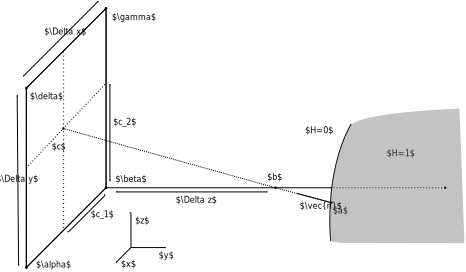
\includegraphics{gfx/immersed_boundary/hpflow/theo/ip.pdf}\label{fig:hpflow_ipgc_theo}
  \caption{blabla}
\end{figure}

\begin{figure}[!pb]
  \centering
  \includegraphics{gfx/immersed_boundary/hpflow/theo/all.pdf}\label{fig:hpflow_allgc_theo}
  \caption{blabla}
\end{figure}

\newpage

For all methods an approximately linear decrease  can be observed.
The error of volume penalizations methods decrease from the order $1e-1$ to $2e-3$, with
a convergence rate of order  $\epsilon \propto N^{\approx1.16}$
The volume fraction methods results in a slighty better convergence rate of $\approx 1.65$.
The overall error is smaller, due to the faster converge rates and of order $5e-4$ for the
highest resolution. For all methods the error is in the order of $1e-2$, above a resolution of 100 points.
The best results are achieved for the 2nd order volume fraction method, except for the highest resolution.\\
Fig. () shows the error of the Direct Forcing method with and without the volume fraction method for 2nd
and 4th order. The error convergence is almost identical to the volume penalization method, when not using the volume
fraction method, of the order $\approx 1.2$. The convergence of the volume fraction methods is of order $\approx 1.45$
and therefore slighly weaker the for the volume penalization method.
As before the best error convergence is given by the volume fraction methond of 2nd order.\\
In Fig. (X) we can see the error convergence of the interpolation schemes.
Here we used 2nd and 4th order schemes, furthermore we compare the interpolation with and without the
use of the direct forcing method.
The 4th order interpolation with direct forcing is not shown, since the resulting velocity fields are becoming
numerically unstable. The 4th order interpolation without DF also results into a larger error but in this case
the velocity field seems to be stable \footnote{This behaviour will be discussed in more detail in section ()}, the
convergence rate is of order $\approx 1.4$ and the error in the regime $1e-1$ to $4e-3$.
The best and furthermore identical results are achieved for the 2nd order interpolation with and without
use of the direct forcing method. The convergence rate is of order $\approx 2.35$ and the error
decreases from the order $2e-2$ to $1e-5$. The identy of these methods occurs due to the decoupling of the velocity fields
on the border ot the fluid domain. Since the interpolation stencil seperates the fluid and wall domain, the 2nd order
stencil doesn't see any points in the wall domain, therefore there is no difference in using the direct forcing method.\\
Finally Fig. () shows the previous methods with the best convergence rates in one plot.
In summary we can say that the overall converges rate of the interpolation method is of one order better
than the volume and direct forcing methods with volume fraction. Furthermore the relative error of the interpolation method ranges
between one and two order of magnitudes below all other methods, depending on the resolution.
The grid convergence study was than repeated once again in order to test the influence of the sound speed with $c^2 = 400$.
As a result it turned out that for all methods the difference in the relative $l_2$-error can be neglected, except
for the 4th order interpolation schemes, in this case the overall error grows. An exemplary plot which compares
the error can be found in Appendix in Fig. (). This behaviour indicates that when using the interpolation with 4th order
an error is induced which is proportional to $c^2\nabla \rho$.\\
As we allready could observe in section (), each immersed boundary method does not converge against the exact theoretical solution.
Therefore, for each method, a grid convergence study was peformed where the theoretical solution is given by a
high resolution solution of each method with $N=512$ points. This type of grid convergence study is often proposed
when no theoretical solution of the fluid problem can be achieved (SOURCE).
For this kind of grid convergence study the numerical setup is similar to the previous one with exeption of the resolution.
Here we use $N\in\{16, 32, 64, 128, 256\}$ for the number of grid points.
The problem occuring with other types of resolution is the position of grid points, which would not exactly overlap anymore with
the high resolution grid  of the theoretical solution of $N=512$.
An alternative would be to use interpolation methods for the exact positions, but the possible disadvantage with these method
would be an additional error resulting from the interpolation scheme.\\
The results of the error analysis are shown in Fig. () (a), exemplarly for the volume penalization, direct forcing  methods with volume fraction
and the interpolation method.

\begin{figure}[!pb]
  \centering
  \includegraphics{gfx/immersed_boundary/hpflow/hd/all.pdf}\label{fig:hpflow_allgc_theo}
  \caption{blabla}
\end{figure}

The convergence rate of the volume penalization method and direct forcing method are of order $\approx 1.44$ and $\approx 1.6$.
Since the finite difference methods are of 2nd order, one would expect a similar decrease in the error.
However we can explain this behaviour by having a look at the velocity profile substracted from the theoretical solution.
Fig. () (b) shows this exemplarly for the direct forcing volume fraction method. It can be noted that
the error vanishes in the middle section of the fluid error whereas the largest differences occur at the fluid domain border.
Therefore we propose that the bad convergence is caused by different approximations of the wall region for different resolutions.
Since the boundary is not mimiced exactly but approximated by the nearest neighboor points in the wall domain, the actual position
of the boundary is dependent of the resolution.\\
The interpolation method of 4th order converges with a rate of $\approx 1.4$ order. It is therefore even worse than the volume penalization and
direct forcing method, altough the overall error is smaller for lower resolutions. Again one possible explanation would be the different rasterization
of the domain border, which does not affect the velocity profiles due to the interpolation but the coupling of the pressure.\\
The 2nd order interpolation method converges is of order $\approx 2.35$, which is better than the expected order of two.
The fluid domain is interpolated at the same positions and since no pressure coupling over the fluid wall occurs the induced error is small.


\subsubsection{Long-Term Simulations}

In Order to test the  numerical stability, additionally a long-term simulation was performed for each IBM.
Again a Reynolds number of $Re=100$ was chosen, with a fixed resolution of $N=96$ grid points.


\begin{figure}[!pt]
  \centering
  \includegraphics{gfx/immersed_boundary/hpflow/long/rho.pdf}\label{fig:hpflow_allgc_theo}
  \caption{blabla}
\end{figure}

\newpage

\begin{figure}[!pb]
  \centering
  \includegraphics{gfx/immersed_boundary/hpflow/long/ts.pdf}\label{fig:hpflow_allgc_theo}
  \caption{blabla}
\end{figure}

\clearpage


